\chapter{Exercise 1}
\begin{comment}
\section{Goal}
The objective of this exercise was to investigate several classical computer vision techniques using thermal and RGB images captured by a drone. The exercise focused on panorama stitching, feature matching across different image modalities, camera calibration, and estimation of the drone's relative motion. In addition to implementing the algorithms, their performance and limitations were evaluated on the provided datasets.

\section{Procedure}
Describe the procedure here.

\section{Results}
Summarize results.
\end{comment}

\section{Introduction}

This chapter summarizes the implementation and evaluation of several computer vision algorithms using the drone image datasets provided. The implemented methods include panorama stitching, feature matching, camera calibration, and extrinsic pose estimation.


\section{Panorama Stitching}

Panorama stitching was performed using OpenCV's built-in \texttt{Stitcher} class. The implementation is shown in Program~\ref{prog:stitch} and Program~\ref{prog:stitch_thermal}.

\begin{program}[H]
\caption{Panorama stitching using OpenCV}
\label{prog:stitch}
\begin{verbatim}
stitcher = cv2.Stitcher_create()

_, panorama = stitcher.stitch(images["RGB"])

imshow(panorama)
\end{verbatim}
\end{program}

\begin{figure}[H]
    \centering
    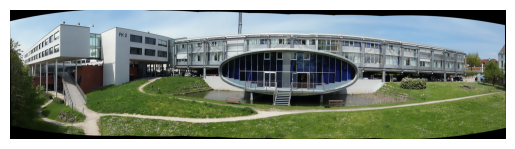
\includegraphics[width=\textwidth]{images/panorama_rgb.png}
    \caption{Panorama generated from the RGB images.}
\end{figure}

\begin{program}[H]
\caption{Thermal panorama stitching}
\label{prog:stitch_thermal}
\begin{verbatim}
_, panorama = stitcher.stitch(images["Thermal"])

imshow(panorama)
\end{verbatim}
\end{program}

\begin{figure}[H]
    \centering
    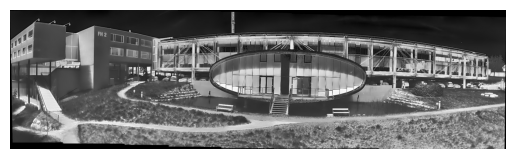
\includegraphics[width=\textwidth]{images/panorama_thermal.png}
    \caption{Panorama generated from the thermal images.}
\end{figure}

The panorama was successfully generated for both the RGB and thermal image sets. The resulting panoramas show that the provided image sequence contains sufficient overlap for automatic image alignment.


\section{Feature Matching}

To compare feature descriptors for thermal and RGB images, SIFT, ORB, and AKAZE were evaluated on all four provided datasets. The features were detected independently in both images, matched using a brute-force matcher, and filtered using the Lowe ratio test. The number of detected keypoints and the remaining good matches were recorded for each descriptor.

\begin{program}[H]
\caption{Feature detection and matching}
\label{prog:feature_matching}
\begin{verbatim}
thermal = cv2.cvtColor(images["Thermal"][0], cv2.COLOR_BGR2GRAY)
rgb = cv2.cvtColor(images["RGB"][0], cv2.COLOR_BGR2GRAY)

kp_t, des_t = detector.detectAndCompute(thermal, None)
kp_r, des_r = detector.detectAndCompute(rgb, None)

bf = cv2.BFMatcher(norm_type)
matches = bf.knnMatch(des_t, des_r, k=2)

good_matches = []
for m, n in matches:
    if m.distance < 0.75 * n.distance:
        good_matches.append(m)
\end{verbatim}
\end{program}

The same procedure was applied to all four scenes using the SIFT, ORB, and AKAZE descriptors. The resulting number of key points detected and good matches is summarized in Table~\ref{tab:feature_matching}.

\begin{table}[H]
    \centering
    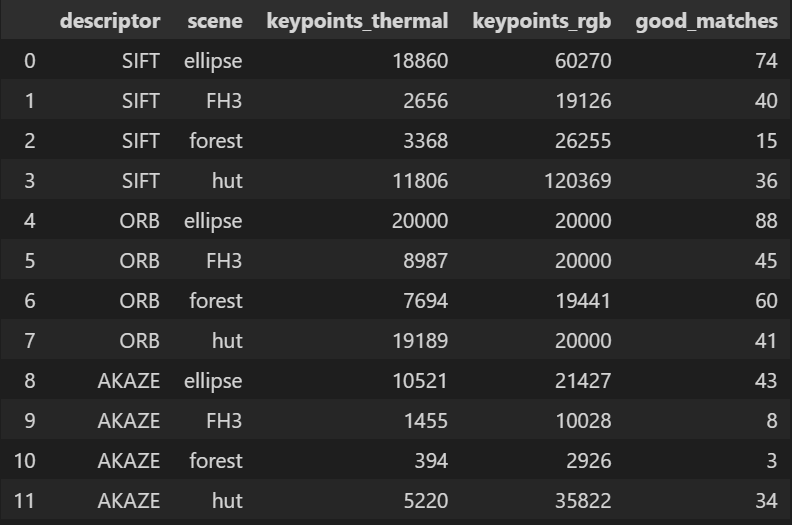
\includegraphics[width=0.8\textwidth]{images/feature_matching.png}
    \caption{Comparison of feature descriptors on the four datasets.}
    \label{tab:feature_matching}
\end{table}

ORB and SIFT produced the most useful results. ORB generated the highest number of good matches after increasing the maximum number of detected features, while SIFT provided stable results with fewer features. AKAZE produced fewer correspondences in all scenes. The quality of the matches should be evaluated not only by the number of matches, but also by the ratio of good matches and by geometric verification using RANSAC inliers.

\section{Camera Calibration}

Camera calibration was performed using the provided chessboard images, as the scene images are not suitable for intrinsic calibration. Chessboard corners were detected and refined before estimating the intrinsic camera parameters and distortion coefficients with OpenCV's calibration functions. To determine the influence of the number of calibration images, the calibration was repeated with an increasing number of images.

\begin{program}[H]
\caption{Camera calibration using chessboard images}
\label{prog:calibration}
\begin{verbatim}
found, corners = cv2.findChessboardCorners(gray, chessboard_size)

if found:
    corners = cv2.cornerSubPix(
        gray, corners, (11,11), (-1,-1), criteria
    )

    object_points.append(objp)
    image_points.append(corners)

error, K, dist, _, _ = cv2.calibrateCamera(
    object_points,
    image_points,
    gray.shape[::-1],
    None,
    None,
)
\end{verbatim}
\end{program}

\begin{program}[H]
\caption{Evaluation of the required number of calibration images}
\label{prog:calibration_evaluation}
\begin{verbatim}
for i in range(2, len(calibration_images) // 2 + 1):
    error, _, _, _, _ = calibrate(calibration_images[:i])
    print(f"Reprojection error with {i} images: {error:.4f} pixels")
\end{verbatim}
\end{program}

\begin{figure}[H]
    \centering
    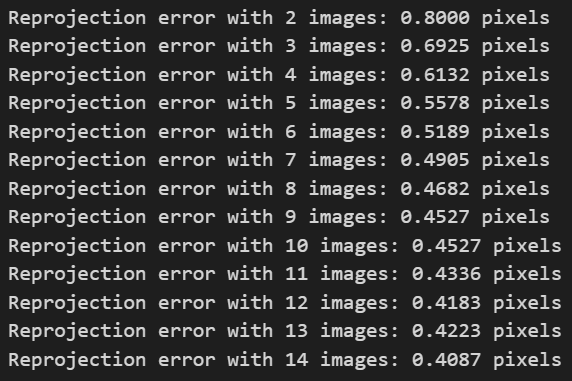
\includegraphics[width=0.8\textwidth]{images/reprojection_error.png}
    \caption{Reprojection error for an increasing number of calibration images.}
    \label{fig:calibration_output}
\end{figure}

Calibration was successful using the provided chessboard images. As shown in Figure~\ref{fig:calibration_output}, at least three images were required to obtain a reliable calibration. Increasing the number of images reduced the reprojection error from 0.6925 pixels to 0.4087 pixels, while the improvement became smaller with additional images.


\section{Extrinsic Estimation}

The relative camera pose was estimated from two consecutive RGB images. SIFT was used to detect and match feature points. The essential matrix was computed using \texttt{findEssentialMat()}, and the relative rotation and translation direction were recovered with \texttt{recoverPose()}. The provided intrinsic camera calibration was used for pose estimation.

\begin{program}[H]
\caption{Relative pose estimation}
\label{prog:pose_estimation}
\begin{verbatim}
sift = cv2.SIFT_create()

kp1, des1 = sift.detectAndCompute(gray1, None)
kp2, des2 = sift.detectAndCompute(gray2, None)

matches = cv2.BFMatcher().knnMatch(des1, des2, k=2)

good_matches = []
for m, n in matches:
    if m.distance < 0.75 * n.distance:
        good_matches.append(m)

E, _ = cv2.findEssentialMat(pts1, pts2, K)

_, R, t, _ = cv2.recoverPose(E, pts1, pts2, K)
\end{verbatim}
\end{program}

\begin{figure}[H]
    \centering
    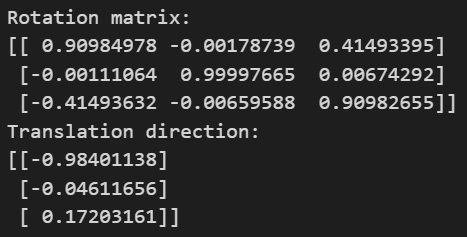
\includegraphics[width=0.60\textwidth]{images/camera_calibration.png}
    \caption{Estimated rotation matrix and translation direction.}
    \label{fig:extrinsic_output}
\end{figure}

The relative rotation and translation direction were successfully estimated. The quality of the estimation depends on the accuracy of the feature matches and can be evaluated using the number of RANSAC inliers.


\section{Conclusion}

The implemented computer vision methods were successfully applied to the drone datasets provided. RGB panorama stitching produced reliable results, while feature matching showed that SIFT and ORB provided the most suitable descriptors for thermal-to-RGB matching. Camera calibration was successfully performed using chessboard images, achieving a low reprojection error. Finally, the relative camera pose was estimated using feature correspondences and the essential matrix.